\documentclass[10pt,letterpaper]{article}
\usepackage[latin1]{inputenc}
\usepackage[margin=1in]{geometry}
\usepackage{amsmath}
\usepackage{amsfonts}
\usepackage{amssymb}
\usepackage{graphicx}
\usepackage{subcaption}
\usepackage{siunitx}

\author{Roy Smart}
\title{EELE 582 Optical Design \\ Final Project Report \\ EUV Solar Telescope Using Fresnel Zone Plates}
\begin{document}
	\maketitle
	
	\section{Introduction}
	
		The Sun is a vibrant source of extreme ultraviolet (EUV) radiation. This radiation is emitted by the million degree solar atmosphere, revealing a complex dynamic structure that is integral to understanding the behavior of the sun and its relationship to the solar system.
		
		Imaging at this wavelength is surprisingly difficult. In the atmosphere, EUV is the most attenuated component of the electromagnetic spectrum and is rarely useful for terrestrial applications. As a result, optical capabilities in this regime are rather primitive compared to that of more familiar regimes such as visible and IR. Further complicating matters, there is non known element or material that is transparent enough to EUV radiation to allow the construction of traditional refractive lenses. Therefore, most EUV optical systems are restricted to reflective optics.
		
		Unfortunately, building reflective optics to operate in EUV remains a difficult and expensive endeavor. Achieving a useful reflection coefficient in this regime requires the use of multilayer coated mirrors. These multilayers are made by depositing multiple alternating, single-atom layers onto a mirror surface. This process results in a reflection coefficient of approximately 30\%, but the process is difficult and there are few vendors with the capability to produce satisfactory multilayer coatings for solar applications.
		
		For this final project we would like to explore an alternative to multilayer reflective optics known as the Fresnel zone plate. This type of lens has a few qualities that make it an attractive tool for use in an EUV imager, such as the ability to mass-produce such a lens for use in an integral field spectrograph for example, and the capability to achieve resolution that would be prohibitive with multilayer coatings.
		
	
	\section{Fresnel Zone Plates}
		
		Unlike traditional optics, Fresnel zone plates rely purely on diffraction to achieve focus. The simplest version of the Fresnel zone plate, a binary zone plate, simply consists of concentric annular rings alternating between fully opaque and fully transparent. These rings are placed such that incoming plane waves of a particular wavelength constructively interfere at the focus.
		
		Noting the geometry given in Figure \ref{fzp}, we define the optical path length
		\begin{equation}
			\ell^2 = r^2 + f^2
			\label{ell}
		\end{equation}
		where $r$ is the radial coordinate measured from the center of the zone plate and $f$ is the desired focal length. To achieve constructive interference at the focus, we need to define the radius at which the difference between the focal length and the path length increases by integer multiples of a half wavelength.
		\begin{equation}
			\frac{(n-1)\lambda}{2} < \ell - f < \frac{n \lambda}{2}
		\end{equation}
		The radii at which the zones should switch between opaque and transparent is found by plugging in Equation \ref{ell} into the above expression and solving the right-hand side of the inequality for $r$, defining this to be the radius of the $n$th zone $r_n$, we have
		\begin{equation}
			r_n^2 = n \lambda \left( f + \frac{n \lambda}{4} \right).
			\label{rad}
		\end{equation}
		Switching from opaque to transparent at odd zones and switching from transparent to opaque at even zones results in the pattern seen in Figure \ref{fzp}. Notice that this choice is arbitrary, and we could just as easily swap the order to achieve the same result.
		
		Notice that Equation \ref{rad} grows as $\sqrt{n}$. This means that the zones decrease in width as we move out towards the edge of the zone plate. As a result, real zone plates must have hundreds to thousands of zones to achieve any appreciable resolution.
		
		Also note that Equation \ref{rad} is dependent on the wavelength $\lambda$. If we hold the radii constant and vary the wavelength, Equation \ref{rad} implies that there is a focal shift proportional to the wavelength. This behavior is known as chromatic aberration and it is quite severe in a Fresnel zone plate compared to traditional refractive lens systems.
		
		\begin{figure}[h!]
			\centering
			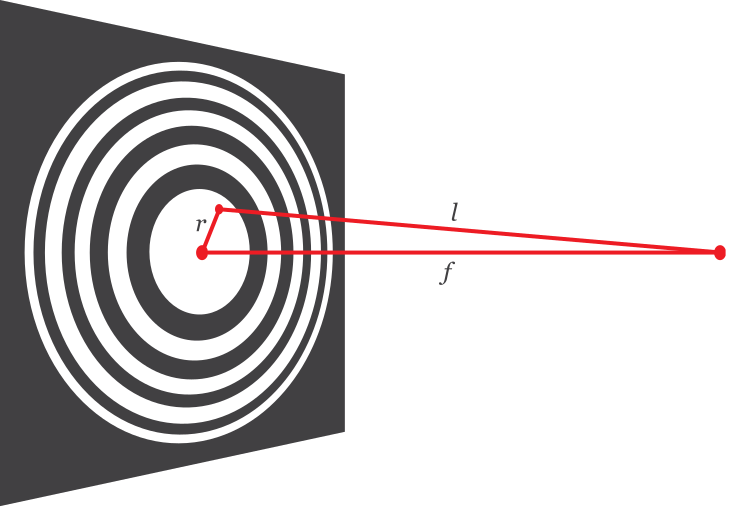
\includegraphics[width=0.6\textwidth]{figures/zone_plate}
			\caption{Visualization and coordinate system of the Fresnel zone plate.}
			\label{fzp}
		\end{figure}
					
	
	\section{EUV Solar Telescope}
		\subsection{Requirements}
			\subsubsection{Resolution}
				Most modern solar observatories, such as the Atmospheric Imaging Assembly (AIA) on board the Solar Dynamics Observatory (SDO) are able to achieve sub-arcsecond resolution (0.6'' in the case of AIA). To be competitive, our zone plate optic should be able to achieve comparable resolution.
			\subsubsection{Passband}
			
				For this project we selected an arbitrary passband encompassing two FeXII emission lines, $\lambda_1 = \SI{193.51}{\angstrom}$ and $\lambda_2 = \SI{195.12}{\angstrom}$, visualized in Figure \ref{spectra}. This passband is likely much narrower than could be achieved with modern EUV filtering technology, but this simple case will serve to demonstrate the chromatic aberration introduced by a zone plate when imaging two characteristic spectral lines. 
			
				\begin{figure}[h!]
					\centering
					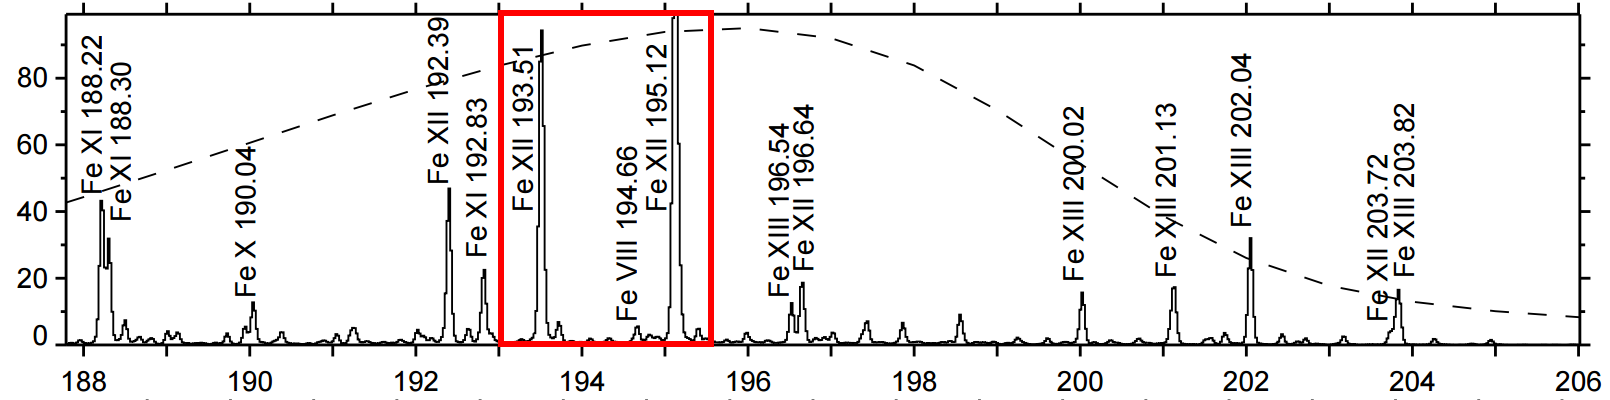
\includegraphics[width=0.9\textwidth]{figures/euv}
					\caption{Sample spectral profile of the Sun between 188 and 206 Angstroms. The passband for our instrument is outlined in red.}
					\label{spectra}
				\end{figure}
				
			\subsubsection{Field of View}
			
				With this instrument, we would like to image the full disk of the sun. This eliminates the need for pointing, and allows us to capture all of the information from the Sun's surface. The Sun has an angular diameter of 0.53 degrees, so we will have field angles of $\alpha = 0.53^\circ / 2 = 0.265$ degrees.
				
			\subsubsection{Detector Size}
			
				For this project, we will choose a 1/2" CCD as our detector, implying an image height $h = 1/4" = \SI{6.35}{\milli \meter}$. This choice is also arbitrary and the real size of the detector will depend on what size EUV CCDs can actually be procured.
			
		\subsection{First-order Design}
		
			With the field of view and image height constrained by the aforementioned requirements, the only remaining free parameter is the focal length $f$. We can find this parameter by solving the triangle
			\begin{align}
				\frac{h}{f} &= \tan \alpha \\
				\Rightarrow f &= \frac{h}{\tan \alpha} \\
				&= \frac{\SI{6.35}{\milli \meter}}{\tan(\SI{0.265}{\deg})} \\
				&= \SI{1373}{\milli \meter}
			\end{align}
			
			With this choice of focal length and choosing to optimize our zone plate around $\lambda_1 = \SI{193.51}{\angstrom}$, we can then use Equation \ref{rad} to find the radius of each zone. For this project we will only model 100 zones of such a zone plate, as simulating larger numbers of zones becomes computationally prohibitive.
		
		\subsection{Zemax Model}
			\subsubsection{Lens Data Editor}
			
				To model our Fresnel zone plate in Zemax, we will define a surface for each opaque zone, located at the origin, and use Zemax's circular obscuration function to make the surface opaque between the appropriate radii, as defined by Equation \ref{rad}. To speed up computation, we also enabled the option \texttt{Use Rays to Propagate to the Next Surface}. This option speeds up computation, since it allows Zemax to understand that each surface is co-spatial.
				
				Entering in the appropriate radii for all 100 zones manually would be vastly time-consuming and if any the parameters are changed, all values would have to be entered in manually again. Therefore to ensure fast and accurate entry of zone surfaces into Zemax, we developed a C++ program that utilizes the Zemax C++ programming interface, that automates the calculation and entry of zone surfaces into the lens data editor. This application proved to be extremely useful, allowing the possibility to test varying focal lengths, wavelengths and different numbers of zones. The result of this program is visualized in Figure \ref{layout}, which shows the 3D layout of the zone plate.
			
				\begin{figure}[h!]
					\centering
					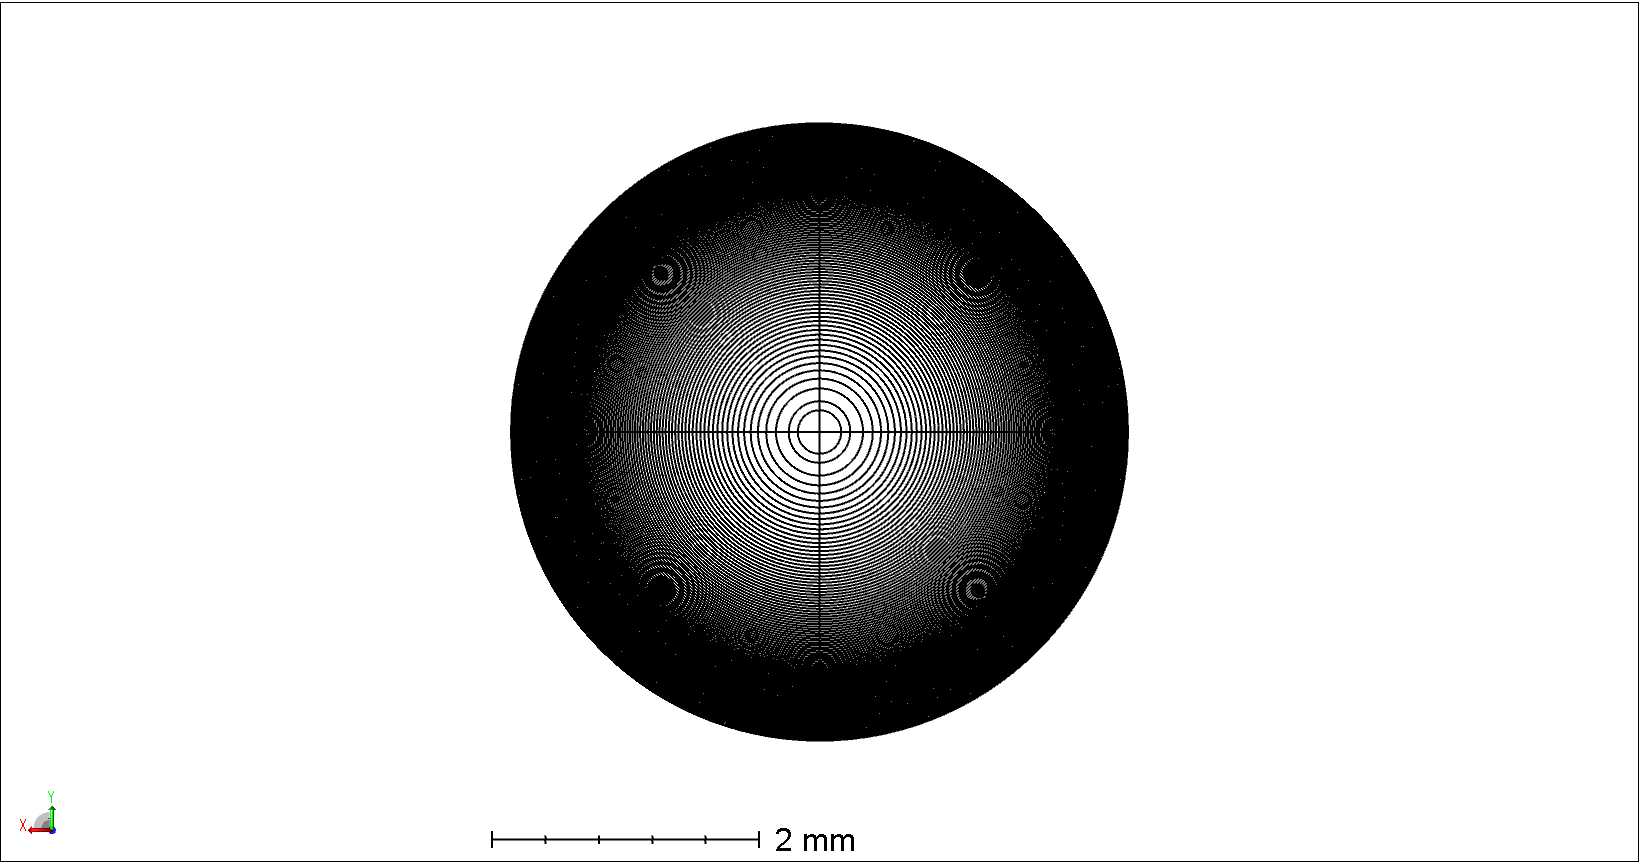
\includegraphics[width=0.8\textwidth]{figures/I90}
					\caption{Layout demonstrating the circular obscurations used to model a zone plate in Zemax}
					\label{layout}
				\end{figure}
			
			\subsubsection{Physical Optics Propagation}
			
				To approximate the optical properties of this Fresnel zone plate lens, we will use Zemax's physical optics propagation (POP) tool. This tool defines a grid on the entrance pupil of the model, and illuminates this grid with beam defined by the user. The POP tool then uses Fresnel diffraction to propagate the beam to the next surface.
				
				To model a point source at infinity representing the Sun, we used the \texttt{Top Hat} beam type to illuminate the aperture of the zone plate. For the square grid, we defined the minimum and maximum values to lie approximately 0.5 mm outside of the outermost zone, and we took the grid size to be $8192\times8192$ points.
				
				In Figure \ref{pop} we can see the results of this physical optics propagation calculation. Figure \ref{pop1} shows the field immediately after the zone plate surface. This figure verifies that the beam is entering the system correctly and that the circular obscurations defined in the previous section are modulating the beam as expected. 
				
				In Figures \ref{pop2} and \ref{pop3} we can see the propagation of the beam at intermediate locations between the aperture and the focus. These figures serve to visualize how light propagates in the system. Here we can see that as light moves past the zone plate, the intensity pattern at the zone plate surface is reproduced and shrunk as we move towards the focus. These two figures also show that the range of our grid is not large enough. Diffracted light is reflected off of the edge of the grid, and results in square waves propagating towards the center of the grid. This effect is obviously unphysical, and could be reduced by changing the minimum and maximum value of the grid. However, we claim that this effect is small, and we are better served by keeping the range of the grid small, allowing for more resolution at the focus.
				
				In Figure \ref{pop4} most of the field is concentrated in a single pixel located at the focus. This figure is taken to be the point-spread function (PSF) of the instrument and will be discussed in detail in the next section.
			
				\begin{figure}[h!]
					\centering
					\begin{subfigure}[t]{0.49\textwidth}
						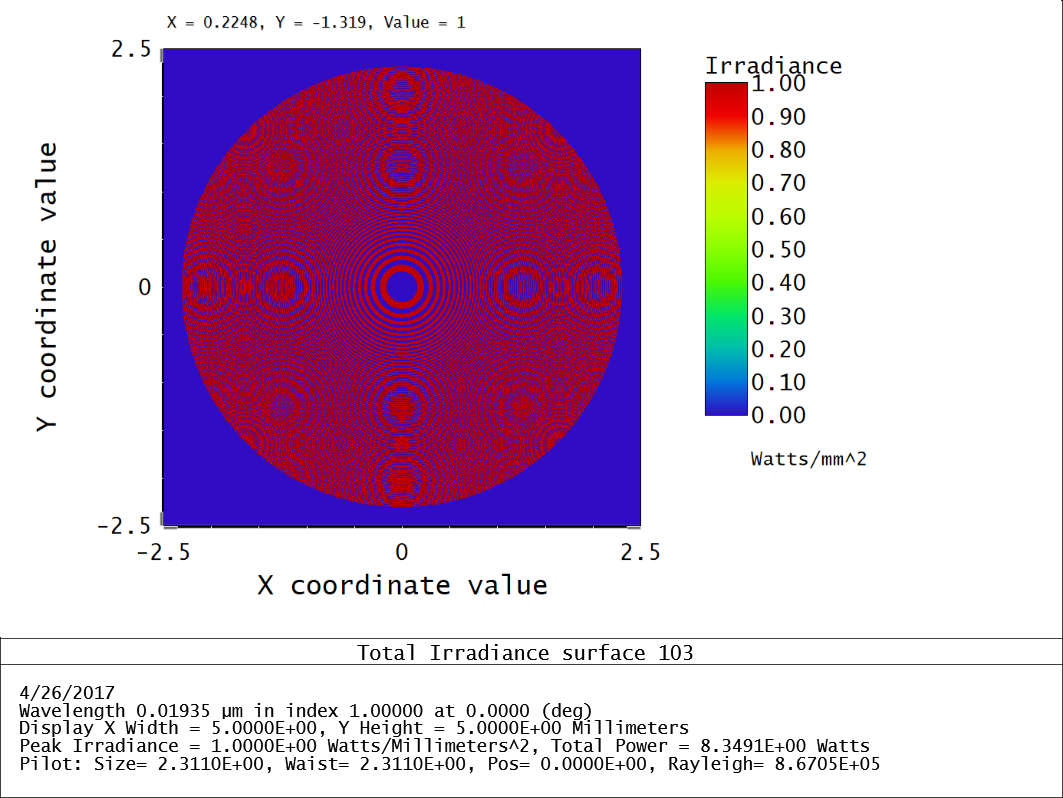
\includegraphics[width=\textwidth]{pop/pop103}
						\caption{Field at aperture}
						\label{pop1}
					\end{subfigure}
					~
					\begin{subfigure}[t]{0.49\textwidth}
						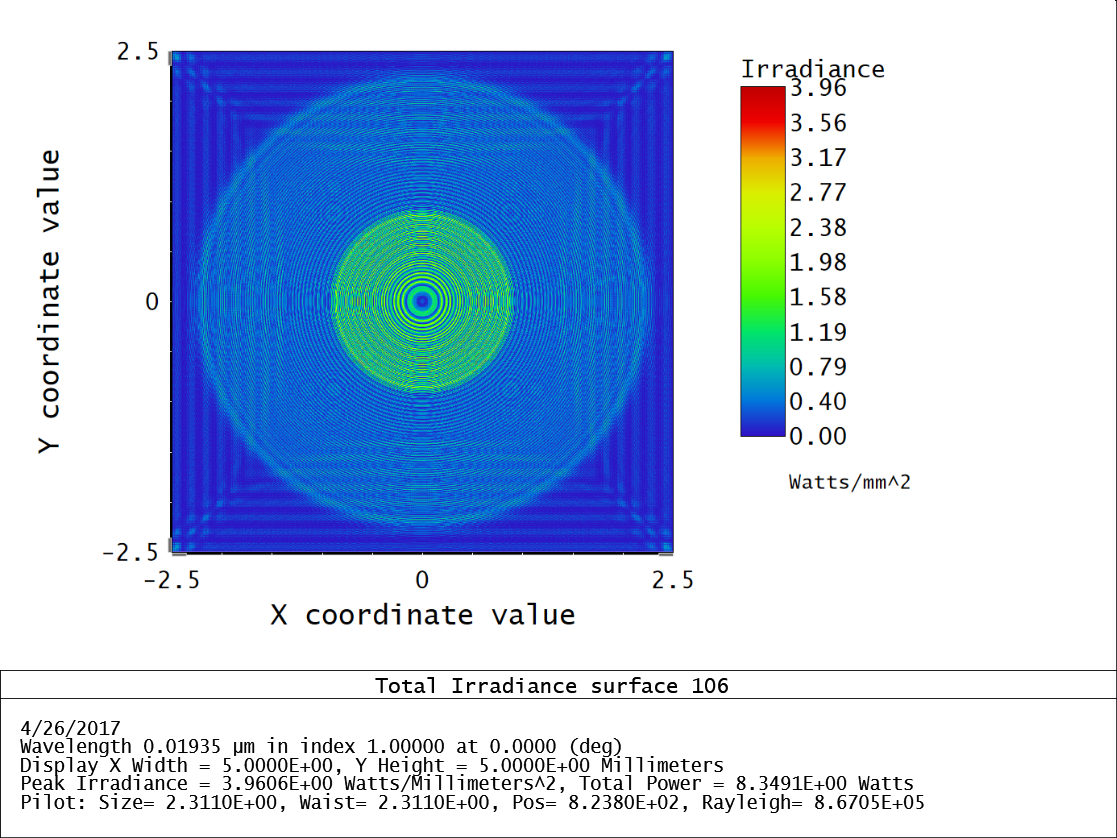
\includegraphics[width=\textwidth]{pop/pop106}	
						\caption{Field at 829 mm behind the aperture}
						\label{pop2}
					\end{subfigure}
					\begin{subfigure}[t]{0.49\textwidth}
						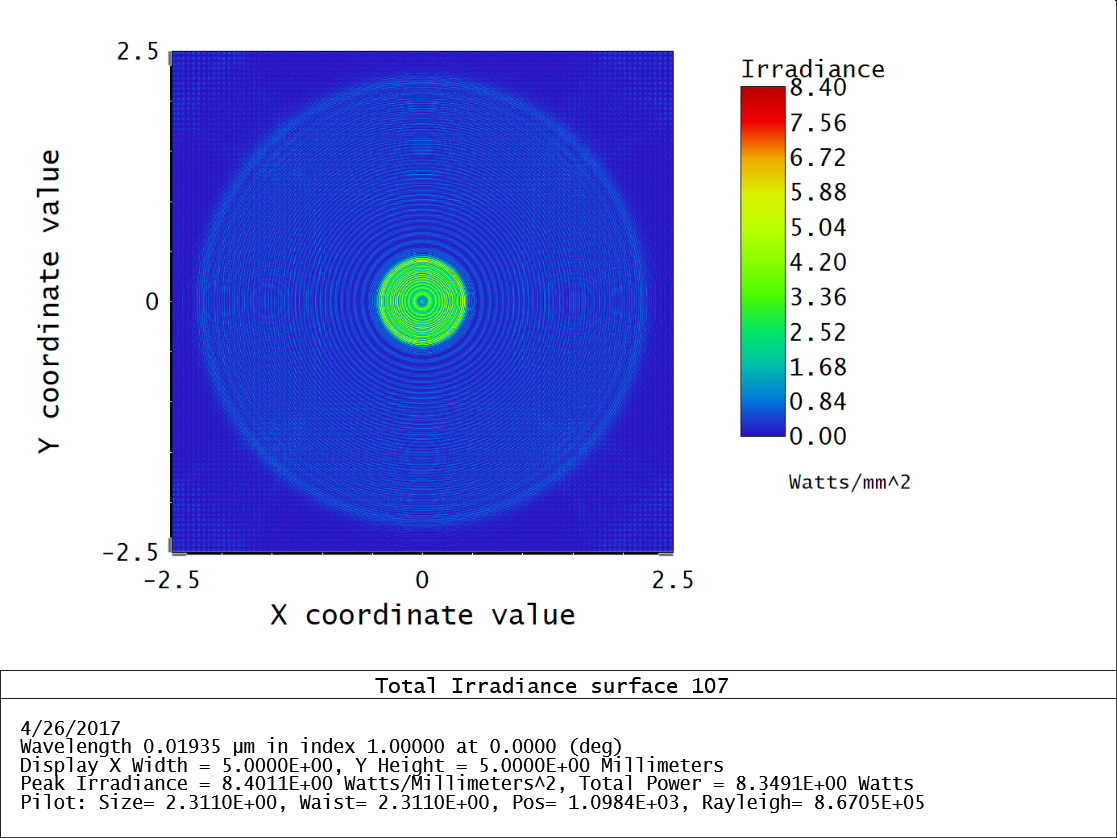
\includegraphics[width=\textwidth]{pop/pop107}
						\caption{Field at 1098 mm behind the aperture}
						\label{pop3}
					\end{subfigure}
					~
					\begin{subfigure}[t]{0.49\textwidth}
						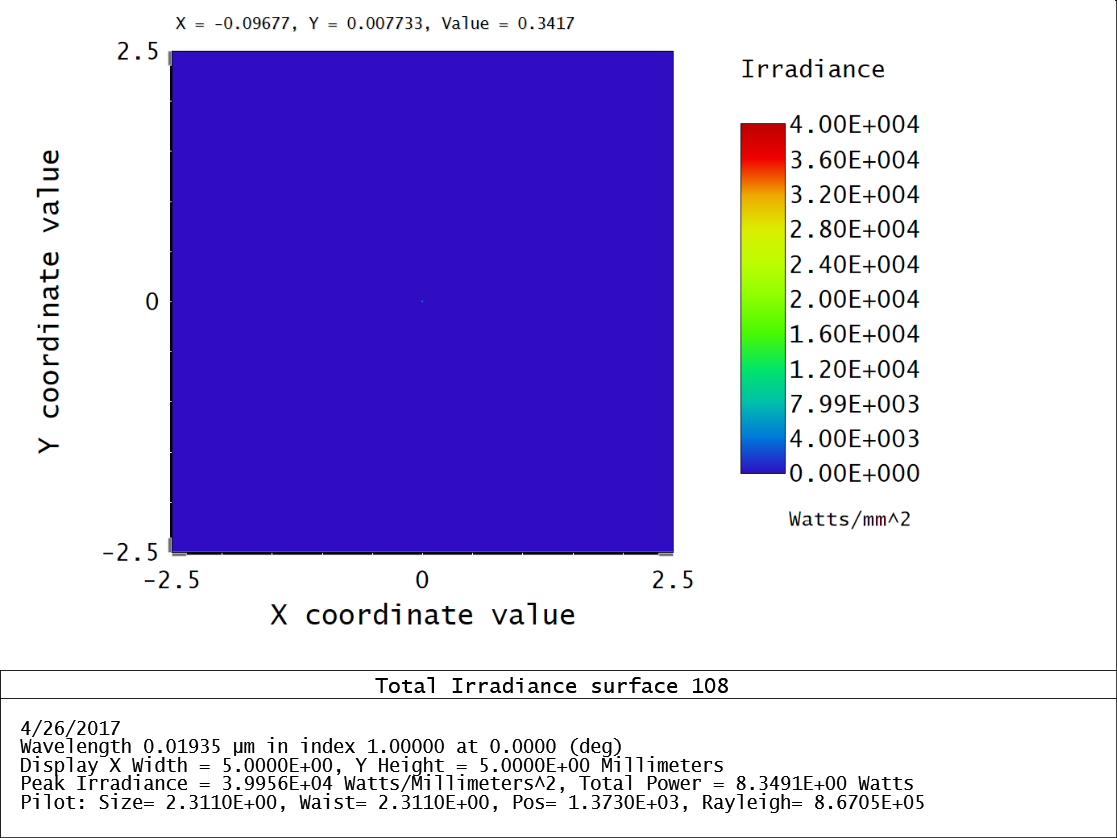
\includegraphics[width=\textwidth]{pop/pop108}	
						\caption{Field at the focus}
						\label{pop4}
					\end{subfigure}
					\caption{Results of physical optics propagation at various locations behind the zone plate surface.}
					\label{pop}
				\end{figure}
			
		\subsection{Performance}
			\subsubsection{Point-spread Function}
			
				\begin{figure}[h!]
					\centering
					\begin{subfigure}[t]{0.49\textwidth}
						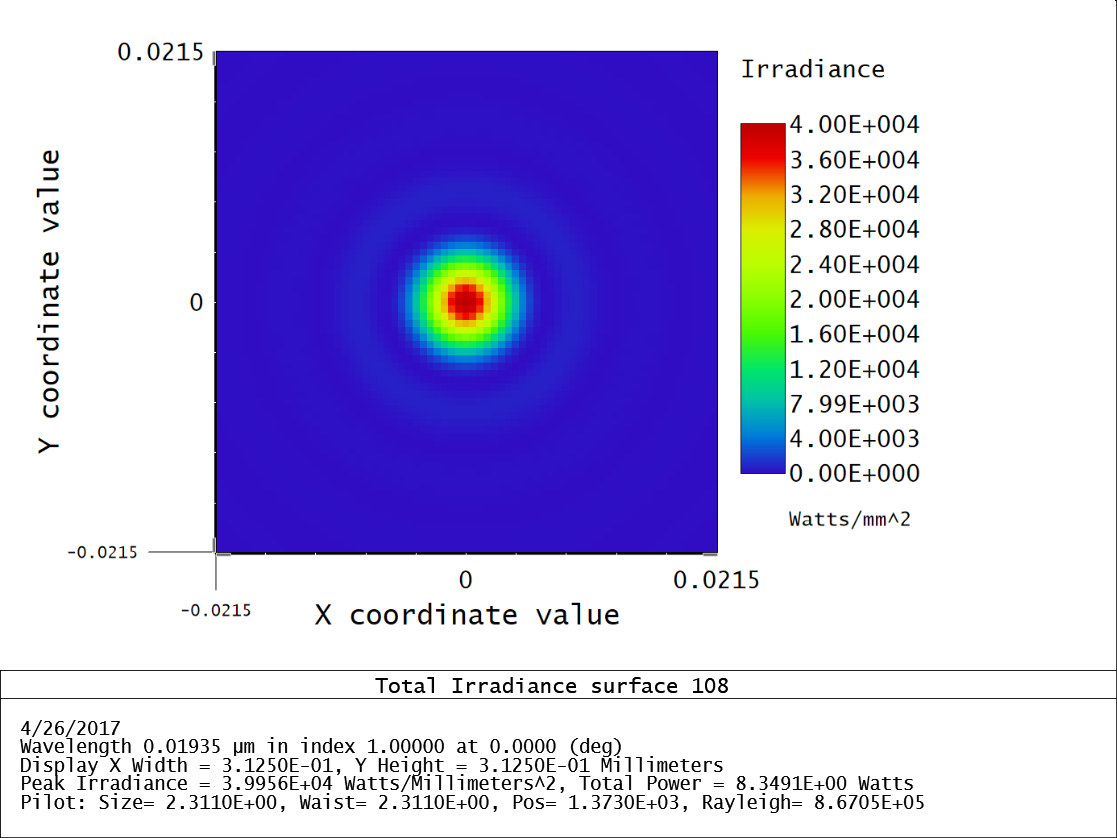
\includegraphics[width=\textwidth]{pop/pop108_zoom2}
						\caption{PSF of the instrument at \SI{193}{\angstrom}}
						\label{psf193}
					\end{subfigure}
					~
					\begin{subfigure}[t]{0.49\textwidth}
						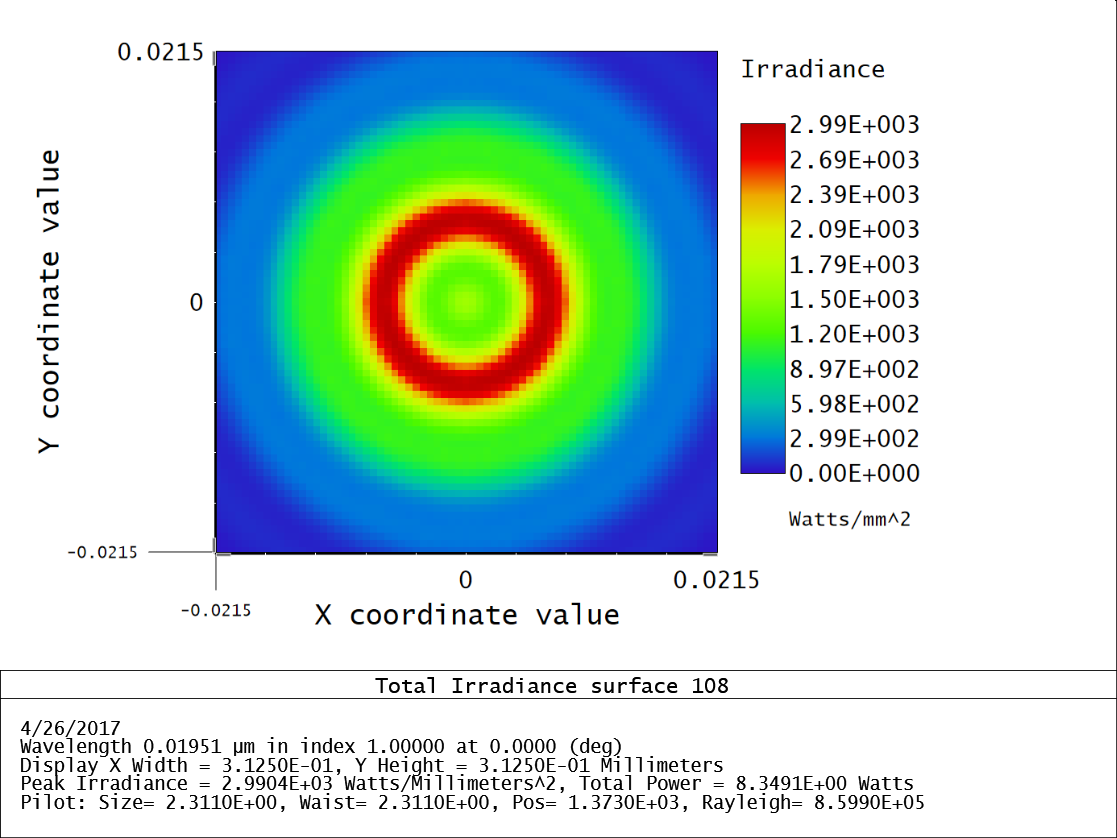
\includegraphics[width=\textwidth]{pop/pop108_zoom2_195}	
						\caption{PSF of the instrument at \SI{195}{\angstrom}}
						\label{psf195}
					\end{subfigure}
					\caption{Results of physical optics propagation at various locations behind the zone plate surface.}
					\label{psf}
				\end{figure}
			
				To calculate the PSF of this instrument, we would have liked to use the FFT or even the Huygens PSF tool implemented in Zemax. Unfortunately, these tools had very unstable behavior when applied to the zone plate system. Both tools were unable to predict the correct PSF size based on the diffraction limit, and returned extremely different results depending on the grid size and number of zones used. Therefore, we used the results of the POP tool to characterize the PSF.
				
				Using the POP tool, we took a zoomed in version of Figure \ref{pop4} to be the PSF for the \SI{193}{\angstrom} line, shown in Figure \ref{psf193}. Performing a similar calculation to the one seen in Figure \ref{pop}, we also obtained a PSF for the \SI{195}{\angstrom} line, seen in Figure \ref{psf195}. The \SI{193}{\angstrom} PSF is diffraction limited (by definition), and has an angular size of approximately 1 arcsecond. The \SI{195}{\angstrom} PSF represents the defocus incurred by the chromatic aberrations of the zone plate, and has a much larger angular size.
			

			
			\subsubsection{Image Simulation}
			
				An important aspect of this project was understanding what the imaging quality of a Fresnel zone plate telescope is, considering the severe chromatic aberrations. Normally, we would've used Zemax's image simulation tool, but unfortunately this tool uses Huygens PSF to perform the simulation. As discussed in the preceding sections, the Huygens PSF tool is unstable for this application. Therefore, to perform our image simulation, we exported the PSF results from the POP calculation to Mathematica, and wrote a simple script to convolve the PSF with some input image.
				
				For this image simulation we will use SDO/AIA images to represent the Sun. We will take the \SI{171}{\angstrom} AIA channel to be a proxy for the \SI{193}{\angstrom} component of our passband, and the \SI{193}{\angstrom} AIA channel to be the proxy for the \SI{195}{\angstrom} component of the passband. The results of the image simulation are shown in Figure \ref{img}.
			
			
				\begin{figure}[h!]
					\centering
					\begin{subfigure}[t]{0.49\textwidth}
						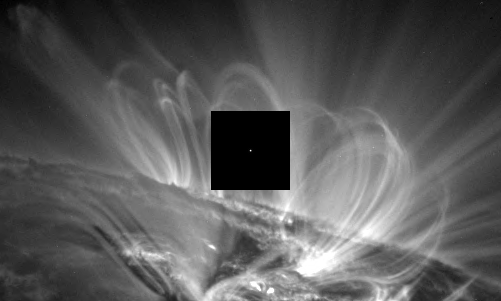
\includegraphics[width=\textwidth]{psf/193/sunAndPsf}
						\caption{\SI{193}{\angstrom} input image with PSF overlay}
						\label{193a}
					\end{subfigure}
					~
					\begin{subfigure}[t]{0.49\textwidth}
						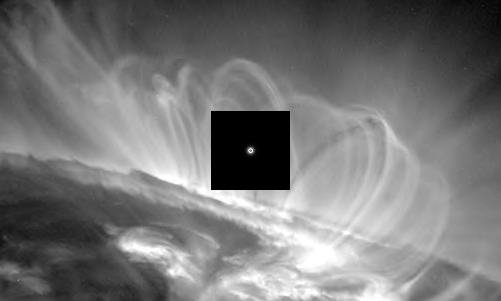
\includegraphics[width=\textwidth]{psf/195/sunAndPsf}	
						\caption{\SI{195}{\angstrom} input image with PSF overlay}
						\label{195a}
					\end{subfigure}
					\begin{subfigure}[t]{0.49\textwidth}
						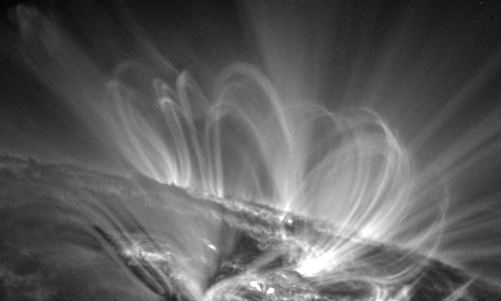
\includegraphics[width=\textwidth]{psf/193/sun}
						\caption{\SI{193}{\angstrom} input image}
						\label{193b}
					\end{subfigure}
					~
					\begin{subfigure}[t]{0.49\textwidth}
						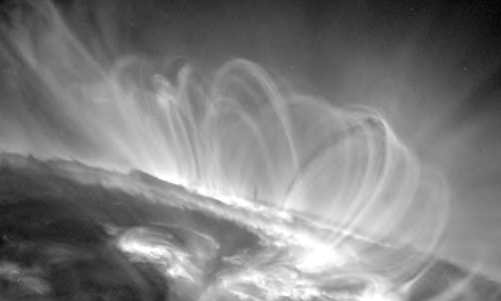
\includegraphics[width=\textwidth]{psf/195/sun}	
						\caption{\SI{195}{\angstrom} input image}
						\label{195b}
					\end{subfigure}
					\begin{subfigure}[t]{0.49\textwidth}
						
\includegraphics[width=\textwidth]{psf/193/img}
						\caption{\SI{193}{\angstrom} input image with PSF applied}
						\label{193c}
					\end{subfigure}
					~
					\begin{subfigure}[t]{0.49\textwidth}
						
\includegraphics[width=\textwidth]{psf/195/img}	
						\caption{\SI{195}{\angstrom} input image with PSF applied}
						\label{195c}
					\end{subfigure}
					\begin{subfigure}[t]{0.51\textwidth}
						
\includegraphics[width=\textwidth]{psf/sum}	
						\caption{Sum of Figures \ref{193c} and \ref{195c}, the observed intensity}
						\label{sum}
					\end{subfigure}
					\caption{Results of image simulation at various steps in the process.}
					\label{img}
				\end{figure}
		
	\section{Conclusion}
	
		In this project, we have nearly accomplished our goal of developing a sub-arcsecond solar EUV telescope using a Fresnel zone plate. While our resolution performance was over 1 arcsecond (barely), we were satisfied by the performance of the zone plate considering the number of zones we attempted to model. Furthermore, we were able to characterize the chromatic aberration present in the zone plate when imaging two closely-spaced, high intensity emission lines. Modeling this chromatic aberration is important as it serves to inform the design of future instruments based off of Fresnel zone plates.
		
		For this project we found the Zemax wasn't really the appropriate tool for zone plate analysis. This is because Zemax does physical optics propagation on a square grid. This square grid is ill-suited to representing zone plates, since the width of the zones quickly decreases as the zone plate is made larger, necessitating grids that would be computationally prohibitive for large zone plates. For future models, we will likely adapt an analytic solution to the field produced by the zone plate, to estimate the PSF and other quantities.
	
\end{document}